% !TEX TS-program = pdflatexmk
\documentclass[12pt]{article}

% Layout.
\usepackage[top=.75in, bottom=0.75in, left=.75in, right=.75in, headheight=1in, headsep=6pt]{geometry}

% Fonts.
\usepackage{mathptmx}
\usepackage[scaled=0.86]{helvet}
\renewcommand{\emph}[1]{\textsf{\textbf{#1}}}

% Misc packages.
\usepackage{amsmath,amssymb,latexsym}
\usepackage{graphicx,tikz}
\usepackage{array}
\usepackage{xcolor}
\usepackage{multicol}
\usepackage{tabularx,colortbl}
\usepackage{enumitem}
%to make tikz pics work
\usepackage{tikz,pgfplots}

\usepackage[colorlinks=true]{hyperref}

% Paragraph spacing
\parindent 0pt
\parskip 6pt plus 1pt
\def\tableindent{\hskip 0.5 in}
\def\ts{\hskip 1.5 em}

\usepackage{fancyhdr}
\pagestyle{fancy} 
\lhead{\large\sf\textbf{MATH 663 }}
\rhead{\large\sf\textbf{Fall 2023}}
\chead{\large\sf\textbf{LaTeX \& Pics}}

\newcommand{\localhead}[1]{\par\smallskip\textbf{#1}\nobreak\\}%
\def\heading#1{\localhead{\large\emph{#1}}}
\def\subheading#1{\localhead{\emph{#1}}}

%% Special Math Symbol shortcuts
\newcommand{\bbN}{\mathbb{N}}
\newcommand{\rad}{\text{rad}}
\newcommand{\diam}{\text{diam}}

%\newenvironment{clist}%
%{\bgroup\parskip 0pt\begin{list}{$\bullet$}{\partopsep 4pt\topsep 0pt\itemsep -2pt}}%
%{\end{list}\egroup}%

\usetikzlibrary{calc}
%\pgfplotsset{my style/.append style={axis x line=middle, axis y line=
%middle, xlabel={$x$}, ylabel={$y$}, axis equal }}


\begin{document}
Often we want to draw pictures to supplement our writing, especially in proofs or in examples. A note of caution that your written words *should* be sufficient to understand your meaning. It is bad form and bad mathematics to depend upon the picture for your argument. Indeed, it is easy to be wrong if you depend too much on a picture. On the other hand, a good picture frequently aids understanding for the reader.

One way to add a picture is to draw it by hand, export it (as a pdf, jpeg, or png), and add the picture using \texttt{$\backslash$includegraphics}. \\

In the example below, a picture was produced by Desmos and exported as a PNG file which lives in the same directory and the TEX file to be compiled. 

The syntax is: \texttt{$\backslash$includegraphics[scale=0.2]$\{$pic-2-1.png$\}$}\\

\includegraphics[scale=0.2]{pic-2-1.png}

Via this method, you can also draw something by hand, upload it in an appropriate format, and embed it in your document. \\

Another approach is to use \texttt{TikZ}. You will need to have \texttt{$\backslash$usepackage$\{$tikz$\}$} in your preamble.

The picture below: 


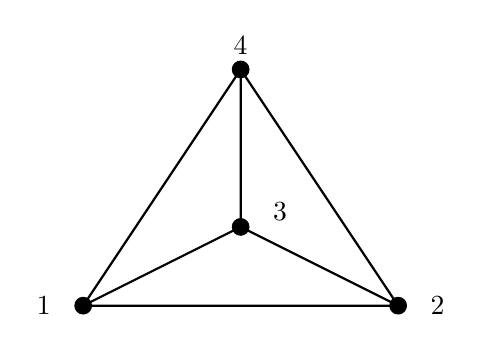
\begin{tikzpicture}
%% vertices
\draw[fill=black] (0,0) circle (3pt);
\draw[fill=black] (4,0) circle (3pt);
\draw[fill=black] (2,1) circle (3pt);
\draw[fill=black] (2,3) circle (3pt);
%% vertex labels
\node at (-0.5,0) {1};
\node at (4.5,0) {2};
\node at (2.5,1.2) {3};
\node at (2,3.3) {4};
%%% edges
\draw[thick] (0,0) -- (4,0) -- (2,1) -- (0,0) -- (2,3) -- (4,0) -- (2,1) -- (2,3);
\end{tikzpicture}


is produced by the following code:\\

\texttt{
$\backslash$begin$\{$tikzpicture$\}$\\
\%\% vertices\\
$\backslash$draw[fill=black] (0,0) circle (3pt);\\
$\backslash$draw[fill=black] (4,0) circle (3pt);\\
$\backslash$draw[fill=black] (2,1) circle (3pt);\\
$\backslash$draw[fill=black] (2,3) circle (3pt);\\
\%\% vertex labels\\
$\backslash$node at (-0.5,0) $\{$1$\}$;\\
$\backslash$node at (4.5,0) $\{$2$\}$;\\
$\backslash$node at (2.5,1.2) $\{$3$\}$;\\
$\backslash$node at (2,3.3) $\{$4$\}$;\\
\%\% edges
$\backslash$draw[thick] (0,0) -- (4,0) -- (2,1) -- (0,0) -- (2,3) -- (4,0) -- (2,1) -- (2,3);\\
$\backslash$end$\{$tikzpicture$\}$
}

 \end{document}


